\documentclass[10pt]{article}
\usepackage{graphicx}
\usepackage{amssymb}
\usepackage[fleqn]{amsmath}
\usepackage{nccmath}
\usepackage{cases}
\usepackage{hyperref}
\usepackage{multicol}
\usepackage{tikz}
\usepackage{pgfplots}
\usepackage{enumitem}
\usepackage{pdfpages}
\pgfplotsset{compat=1.18}
\usepackage{float}


\title{\bf Math 151b: Problem Set 7}
\date{3/6/2024}
\author{\bf Owen Jones}
\begin{document}
\maketitle

\noindent\textbf{Problem 1}\\
\begin{enumerate}[label=(\alph*)]
   \item Case 1: $\mathbf{v}=\mathbf{0}$\\
   Trivially $\lVert A\mathbf{v}\rVert=\lVert \mathbf{0}\rVert=0\le 0=\lVert\mathbf{A}\rVert 0=\lVert A\rVert \cdot\lVert\mathbf{v}\rVert$\\
   Case 2: $\mathbf{v}\neq\mathbf{0}$\\
   Let $\mathbf{w}=\frac{\mathbf{v}}{\lVert\mathbf{v}\rVert}\Rightarrow\lVert\mathbf{w}\rVert=1$.\\
   $\lVert A\mathbf{w}\rVert\le\underset{\lVert\mathbf{x}\rVert=1}{\max}\lVert A\mathbf{x}\rVert=\lVert A\rVert\Rightarrow \lVert A\mathbf{w}\rVert\le\lVert A\rVert$.\\
   Thus, $\lVert A\mathbf{w}\rVert=\lVert A\frac{\mathbf{v}}{\lVert\mathbf{v}\rVert}\rVert=\frac{1}{\lVert\mathbf{v}\rVert}\lVert A\mathbf{v}\rVert\le\lVert A\rVert\Rightarrow\lVert A\mathbf{v}\rVert\le\lVert A\rVert\cdot\lVert\mathbf{v}\rVert$.
   \item Suppose $\lVert \mathbf{x}\rVert=1$.\\
   Observe $Range(\mathbf{B})\subset\mathbb{R}^n$.\\
   $\lVert AB\mathbf{x}\rVert\le\lVert A\rVert\cdot\lVert B\mathbf{x}\rVert\le \lVert A\rVert\cdot\lVert B\rVert\cdot\lVert\mathbf{x}\rVert=\lVert A\rVert\cdot\lVert B\rVert$ by part (a).\\
   Since this innequality holds for any $\lVert \mathbf{x}\rVert=1$, the innequality must hold for $\lVert AB\rVert=\underset{\lVert \mathbf{x}\rVert=1}{\max}\lVert AB\mathbf{x}\rVert\le\lVert A\rVert\cdot\lVert B\rVert$.\\
   Thus, $\lVert AB\rVert\le\lVert A\rVert\cdot\lVert B\rVert$.
\end{enumerate}
\textbf{Problem 2}\\
We will prove $\rho(\cdot)$ is not a matrix norm by contrapositive. Let $\mathbf{A}\in\mathbb{R}^{n\times n}\neq\mathbf{0}$ be a strictly triangular matrix. 
Because the eigenvalues of a triangular matrix are the elements along the main diagonal, $\lambda_i=0$, $i=1,\ldots, n$.
It follows $\rho(\mathbf{A})=\underset{1\le i\le n}{\max}\lvert \lambda_i\rvert=0$.
Because $\rho(\mathbf{A})=0\not\Rightarrow \mathbf{A}=\mathbf{0}$, $\rho(\cdot)$ is not a matrix norm.\\
\textbf{Problem 3}\\
$G_j=D^{-1}(L+U),G_g={(D-L)}^{-1} U$\\
$D=\begin{bmatrix}
   2 & 0 & 0\\
   0 & 1 & 0\\
   0 & 0 & 2
\end{bmatrix}, L=\begin{bmatrix}
   0 & 0 & 0\\
   -1 & 0 & 0\\
   1 & 1 & 0
\end{bmatrix}, U=\begin{bmatrix}
   0 & 1 & -1\\
   0 & 0 & -1\\
   0 & 0 & 0
\end{bmatrix}$\\
$G_j=\begin{bmatrix}
   \frac{1}{2} & 0 & 0\\
   0 & 1 & 0\\
   0 & 0 & \frac{1}{2}
\end{bmatrix}\begin{bmatrix}
   0 & 1 & -1\\
   -1 & 0 & -1\\
   1 & 1 & 0
\end{bmatrix}=\begin{bmatrix}
   0 & \frac{1}{2} & -\frac{1}{2}\\
   -1 & 0 & -1\\
   \frac{1}{2} & \frac{1}{2} & 0
\end{bmatrix}$\\
$\begin{bmatrix}
   2 & 0 & 0\\
   1 & 1 & 0\\
   -1 & -1 & 2
\end{bmatrix}^{-1}=
\begin{bmatrix}
   1 & 0 & 0\\
   -1 & 1 & 0\\
   0 & 0 & 1
\end{bmatrix}
\begin{bmatrix}
   1 & 0 & 0\\
   0 & 1 & 0\\
   0 & 0 & \frac{1}{2}
\end{bmatrix}
\begin{bmatrix}
   1 & 0 & 0\\
   0 & 1 & 0\\
   0 & 1 & 1
\end{bmatrix}
\begin{bmatrix}
   \frac{1}{2} & 0 & 0\\
   0 & 1 & 0\\
   0 & 0 & 1
\end{bmatrix}
\begin{bmatrix}
   1 & 0 & 0\\
   0 & 1 & 0\\
   0 & 0 & 1
\end{bmatrix}\\
=\begin{bmatrix}
   \frac{1}{2} & 0 & 0\\
   -\frac{1}{2} & 1 & 0\\
   0 & \frac{1}{2} & \frac{1}{2}
\end{bmatrix}$\\
$G_g=\begin{bmatrix}
   \frac{1}{2} & 0 & 0\\
   -\frac{1}{2} & 1 & 0\\
   0 & \frac{1}{2} & \frac{1}{2}
\end{bmatrix}
\begin{bmatrix}
   0 & 1 & -1\\
   0 & 0 & -1\\
   0 & 0 & 0
\end{bmatrix}=
\begin{bmatrix}
   0 & \frac{1}{2} & -\frac{1}{2}\\
   0 & -\frac{1}{2} & \frac{1}{2}\\
   0 & 0 & -\frac{1}{2}
\end{bmatrix}$\\
\begin{enumerate}[label=(\alph*)]
   \item For $G_j$ $\det(\lambda I-G_j)=\lambda^3+\frac{5}{4}\lambda$, $\lambda=0,\frac{\sqrt{5}i}{2},-\frac{\sqrt{5}i}{2}\\
   \Rightarrow\rho(G_j)=\lvert\frac{\sqrt{5}i}{2}\rvert=\frac{\sqrt{5}}{2}<1$
   \item For $G_g$ eigenvalues are elements along diagonal, $\lambda=0,-\frac{1}{2}\\
   \Rightarrow\rho(G_g)=\lvert-\frac{1}{2}\rvert=\frac{1}{2}<1$
\end{enumerate}
\textbf{Problem 4}\\
\begin{enumerate}[label=(\alph*)]
   \item $G_j=D^{-1}(L+U)=\begin{bmatrix}
      1 & 0 & 0\\
      0 & 1 & 0\\
      0 & 0 & 1
   \end{bmatrix}\begin{bmatrix}
      0 & -2 & 2\\
      -1 & 0 & -1\\
      -2 & -2 & 0
   \end{bmatrix}=\begin{bmatrix}
      0 & -2 & 2\\
      -1 & 0 & -1\\
      -2 & -2 & 0
   \end{bmatrix}$\\
   For $G_j$ $\det(\lambda I-G_j)=\lambda(\lambda^2-2)-2(\lambda-2)+4(\lambda+1)=\lambda^3\\
   \Rightarrow \rho(G_j)=\lvert0\rvert=0<1$
   \item ${(D-L)}^{-1}=\begin{bmatrix}
      1 & 0 & 0\\
      1 & 1 & 0\\
      2 & 2 & 1
   \end{bmatrix}^{-1}=
   \begin{bmatrix}
      1 & 0 & 0\\
      -1 & 1 & 0\\
      0 & 0 & 1
   \end{bmatrix}
   \begin{bmatrix}
      1 & 0 & 0\\
      0 & 1 & 0\\
      0 & -2 & 1
   \end{bmatrix}
   \begin{bmatrix}
      1 & 0 & 0\\
      0 & 1 & 0\\
      0 & 0 & 1
   \end{bmatrix}=\begin{bmatrix}
      1 & 0 & 0\\
      -1 & 1 & 0\\
      0 & -2 & 1
   \end{bmatrix}$\\
   $G_g={(D-L)}^{-1}U=\begin{bmatrix}
      1 & 0 & 0\\
      -1 & 1 & 0\\
      0 & -2 & 1
   \end{bmatrix}\begin{bmatrix}
      0 & -2 & 2\\
      0 & 0 & -1\\
      0 & 0 & 0
   \end{bmatrix}=\begin{bmatrix}
      0 & -2 & 2\\
      0 & 2 & -3\\
      0 & 0 & 2
   \end{bmatrix}$\\
   For $G_g$ eigenvalues are elements along diagonal, $\lambda=0,2\\
   \Rightarrow\rho(G_g)=\lvert2\rvert=2>1$
\end{enumerate}
\textbf{Problem 5}\\
\begin{enumerate}[label=(\alph*)]
   \item Proof by induction:\\
   Base case: $\lVert \mathbf{x}^{(1)}-\mathbf{x}\rVert=\lVert(G\mathbf{x}^{(0)}+c)-(G\mathbf{x}+c)\rVert\\
   =\lVert G(\mathbf{x}^{(0)}-\mathbf{x})\rVert\le\lVert G\rVert\lVert \mathbf{x}^{(0)}-\mathbf{x}\rVert$ by Problem 1.\\
   Induction hypothesis: Assume for some $k$ $\lVert \mathbf{x}^{(k)}-\mathbf{x}\rVert\le {\lVert G\rVert}^k\lVert \mathbf{x}^{(0)}-\mathbf{x}\rVert$.\\
   Induction step: $\lVert \mathbf{x}^{(k+1)}-\mathbf{x}\rVert=\lVert(G\mathbf{x}^{(k)}+c)-(G\mathbf{x}+c)\rVert\\
   =\lVert G(\mathbf{x}^{(k)}-\mathbf{x})\rVert\le\lVert G\rVert\lVert \mathbf{x}^{(k)}-\mathbf{x}\rVert\\
   \le{\lVert G\rVert}^{k+1}\lVert \mathbf{x}^{(0)}-\mathbf{x}\rVert$ by the induction hypothesis.\\
   Hence, by induction, the claim holds for all $k$.
   \item \begin{enumerate}[label=(\roman*)]
      \item Proof by induction:\\
      Base case: $\lVert \mathbf{x}^{(2)}-\mathbf{x}^{(1)}\rVert=\lVert(G\mathbf{x}^{(1)}+c)-(G\mathbf{x}^{(0)}+c)\rVert\\
      =\lVert G(\mathbf{x}^{(1)}-\mathbf{x}^{(0)})\rVert\le\lVert G\rVert\lVert \mathbf{x}^{(1)}-\mathbf{x}^{(0)}\rVert$ by Problem 1.\\
      Induction hypothesis: Assume for some $k$ $\lVert \mathbf{x}^{(k)}-\mathbf{x}^{(k-1)}\rVert\le {\lVert G\rVert}^{k-1}\lVert \mathbf{x}^{(1)}-\mathbf{x}^{(0)}\rVert$.\\
      Induction step: $\lVert \mathbf{x}^{(k+1)}-\mathbf{x}^{(k)}\rVert=\lVert(G\mathbf{x}^{(k)}+c)-(G\mathbf{x}^{(k-1)}+c)\rVert\\
      =\lVert G(\mathbf{x}^{(k)}-\mathbf{x}^{(k-1)})\rVert\le\lVert G\rVert\lVert \mathbf{x}^{(k)}-\mathbf{x}^{(k-1)}\rVert\\
      \le{\lVert G\rVert}^{k}\lVert \mathbf{x}^{(1)}-\mathbf{x}^{(0)}\rVert$ by the induction hypothesis.\\
      Hence, by induction, the claim holds for all $k$.
      \item Proof by induction:\\
      Base case: the base case is proved in part (a). We know $\lVert \mathbf{x}^{(k+1)}-\mathbf{x}^{(k)}\rVert\le{\lVert G\rVert}^{k}\lVert \mathbf{x}^{(1)}-\mathbf{x}^{(0)}\rVert$\\
      Induction hypothesis: Assume for some $m>k$\\
      $\displaystyle\lVert\mathbf{x}^{(m)}-\mathbf{x}^{(k)}\rVert\le{\lVert G\rVert}^{k}\lVert\mathbf{x}^{(1)}-\mathbf{x}^{(0)}\rVert\sum_{i=0}^{m-k-1}{\lVert G\rVert}^{i}$\\
      Induction step: $\lVert \mathbf{x}^{(m+1)}-\mathbf{x}^{(m)}\rVert\le{\lVert G\rVert}^{m}\lVert \mathbf{x}^{(1)}-\mathbf{x}^{(0)}\rVert$ by part (a).\\
      $\lVert \mathbf{x}^{(m+1)}-\mathbf{x}^{(m)}\rVert+\lVert\mathbf{x}^{(m)}-\mathbf{x}^{(k)}\rVert\\
      \le{\lVert G\rVert}^{m-k}{\lVert G\rVert}^{k}\lVert \mathbf{x}^{(1)}-\mathbf{x}^{(0)}\rVert+{\lVert G\rVert}^{k}\lVert\mathbf{x}^{(1)}-\mathbf{x}^{(0)}\rVert\sum_{i=0}^{m-k-1}{\lVert G\rVert}^{i}\\
      ={\lVert G\rVert}^{k}\lVert\mathbf{x}^{(1)}-\mathbf{x}^{(0)}\rVert\sum_{i=0}^{m-k}{\lVert G\rVert}^{i}$.\\
      By the triangle innequality $\lVert\mathbf{x}^{(m+1)}-\mathbf{x}^{(k)}\rVert\le\lVert\mathbf{x}^{(m+1)}-\mathbf{x}^{(m)}\rVert+\lVert\mathbf{x}^{(m)}-\mathbf{x}^{(k)}\rVert$\\
      Thus, $\displaystyle\lVert\mathbf{x}^{(m+1)}-\mathbf{x}^{(k)}\rVert\le{\lVert G\rVert}^{k}\lVert\mathbf{x}^{(1)}-\mathbf{x}^{(0)}\rVert\sum_{i=0}^{m-k}{\lVert G\rVert}^{i}$.\\
      Hence, by induction, the claim holds for all $m$.
      \item Suppose $\lVert G\rVert<1$.\\
      $\lVert \mathbf{x}^{(m)}-\mathbf{x}\rVert\le {\lVert G\rVert}^m\lVert \mathbf{x}^{(0)}-\mathbf{x}\rVert$ from part (a).\\
      It follows $\displaystyle \lim_{m\rightarrow \infty}\lVert\mathbf{x}^{(m)}-\mathbf{x}\rVert=0\Rightarrow \mathbf{x}^{(m)}\rightarrow \mathbf{x}$ as $m\rightarrow \infty$.\\
      Thus, $\displaystyle\lVert\mathbf{x}^{(k)}-\mathbf{x}\rVert=\lim_{m\rightarrow\infty}\lVert\mathbf{x}^{(k)}-\mathbf{x}^{(m)}\rVert$.\\
      $\displaystyle\lVert\mathbf{x}^{(m)}-\mathbf{x}^{(k)}\rVert\le{\lVert G\rVert}^{k}\lVert\mathbf{x}^{(1)}-\mathbf{x}^{(0)}\rVert\sum_{i=0}^{m-k-1}{\lVert G\rVert}^{i}$ from part (b)(ii).\\
      $\displaystyle{\lVert G\rVert}^{k}\lVert\mathbf{x}^{(1)}-\mathbf{x}^{(0)}\rVert\sum_{i=0}^{m-k-1}{\lVert G\rVert}^{i}=\frac{{\lVert G\rVert}^{k}-{\lVert G\rVert}^{m}}{1-\lVert G\rVert}$ for all $m>k$ by the sum of a geometric series.\\
      Using $\lVert G\rVert<1$, $\displaystyle\lim_{m\rightarrow\infty}\frac{{\lVert G\rVert}^{k}-{\lVert G\rVert}^{m}}{1-\lVert G\rVert}=\frac{{\lVert G\rVert}^{k}}{1-\lVert G\rVert}$.\\
      Hence, by the squeeze theorem, $\lVert\mathbf{x}^{(k)}-\mathbf{x}^{(m)}\rVert\le \frac{{\lVert G\rVert}^{k}-{\lVert G\rVert}^{m}}{1-\lVert G\rVert}$ for all $m>k$ implies $\lVert\mathbf{x}^{(k)}-\mathbf{x}\rVert\le\frac{{\lVert G\rVert}^{k}}{1-\lVert G\rVert}$.\\
      (Note: I know the squeeze theorem requires the innequality to hold for every element of the sequence, but we can easily get around that by defining $2$ sequences $A_n:=\lVert\mathbf{x}^{(k)}-\mathbf{x}^{(k+1+n)}\rVert$ and $B_n:=\frac{{\lVert G\rVert}^{k}-{\lVert G\rVert}^{k+1+n}}{1-\lVert G\rVert}$ which satisfy the condition $A_n\le B_n$ for all $n\ge0$).
   \end{enumerate}
\end{enumerate}
\textbf{Problem 6}\\
\begin{enumerate}[label=(\alph*)]
   \item $D=\begin{bmatrix}
      10 & & &\\
      & 10 & &\\
      & & 8 &\\
      & & & 5
   \end{bmatrix},
   L=\begin{bmatrix}
      & & & \\
      -5 & & &\\
      & 4 & &\\
      & & 1 &
   \end{bmatrix},
   U=\begin{bmatrix}
      & -5 & &\\
      & & 4 &\\
      & & & 1\\
      & & &
   \end{bmatrix},
   b=\begin{bmatrix}
      6\\
      25\\
      -11\\
      -11
   \end{bmatrix}$\\
   $G_j=\begin{bmatrix}
      \frac{1}{10} & & &\\
      & \frac{1}{10} & &\\
      & & \frac{1}{8} &\\
      & & & \frac{1}{5}
   \end{bmatrix}\begin{bmatrix}
      & -5 & &\\
      -5& & 4 &\\
      & 4& & 1\\
      & & 1&
   \end{bmatrix}=\begin{bmatrix}
      & -\frac{1}{2} & &\\
      -\frac{1}{2}& & \frac{2}{5} &\\
      & \frac{1}{2}& & \frac{1}{8}\\
      & & \frac{1}{5}&
   \end{bmatrix}$\\
   $c_j=\begin{bmatrix}
      \frac{1}{10} & & &\\
      & \frac{1}{10} & &\\
      & & \frac{1}{8} &\\
      & & & \frac{1}{5}
   \end{bmatrix}\begin{bmatrix}
      6\\
      25\\
      -11\\
      -11
   \end{bmatrix}=\begin{bmatrix}
      \frac{3}{5}\\
      \frac{5}{2}\\
      -\frac{11}{8}\\
      -\frac{11}{5}
   \end{bmatrix}$\\
   $\mathbf{x}_j^{(1)}=G_j\mathbf{x}_j^{(0)}+c_j=c_j=\begin{bmatrix}
      \frac{3}{5}\\
      \frac{5}{2}\\
      -\frac{11}{8}\\
      -\frac{11}{5}
   \end{bmatrix}$\\
   $\mathbf{x}_j^{(2)}=G_j\mathbf{x}_j^{(1)}+c_j=(G_j+I)c_j=\begin{bmatrix}
      1 & -\frac{1}{2} & &\\
      -\frac{1}{2}& 1 & \frac{2}{5} &\\
      & \frac{1}{2}& 1 & \frac{1}{8}\\
      & & \frac{1}{5}& 1
   \end{bmatrix}\begin{bmatrix}
      \frac{3}{5}\\
      \frac{5}{2}\\
      -\frac{11}{8}\\
      -\frac{11}{5}
   \end{bmatrix}=\begin{bmatrix}
      -\frac{13}{20}\\
      \frac{33}{20}\\
      -\frac{2}{5}\\
      -\frac{99}{40}
   \end{bmatrix}$\\
   ${(D-L)}^{-1}=\begin{bmatrix}
      10 & & &\\
      5 & 10 & &\\
      & -4 & 8 &\\
      & & -1 & 5
   \end{bmatrix}^{-1}=
   \begin{bmatrix}
      1 & & &\\
      & 1 & &\\
      & & 1 &\\
      & & & \frac{1}{5}
   \end{bmatrix}
   \begin{bmatrix}
      1 & & &\\
      & 1 & &\\
      & & 1 &\\
      & & 1 & 1
   \end{bmatrix}
   \begin{bmatrix}
      1 & & &\\
      & 1 & &\\
      & & \frac{1}{8} &\\
      & & & 1
   \end{bmatrix}\\
   \begin{bmatrix}
      1 & & &\\
      & 1 & &\\
      & 4 & 1 &\\
      & & & 1
   \end{bmatrix}
   \begin{bmatrix}
      1 & & &\\
      & \frac{1}{10} & &\\
      & & 1 &\\
      & & & 1
   \end{bmatrix}
   \begin{bmatrix}
      1 & & &\\
      -5 & 1 & &\\
      & & 1 &\\
      & & & 1
   \end{bmatrix}
   \begin{bmatrix}
      \frac{1}{10} & & &\\
      & 1 & &\\
      & & 1 &\\
      & & & 1
   \end{bmatrix}=\begin{bmatrix}
      \frac{1}{10} & & &\\
      -\frac{1}{20} & \frac{1}{10} & &\\
      -\frac{1}{40} & \frac{1}{20} & \frac{1}{8} &\\
      -\frac{1}{200} & \frac{1}{100} &\frac{1}{40} & \frac{1}{5}
   \end{bmatrix}$\\
   $G_g=\begin{bmatrix}
      \frac{1}{10} & & &\\
      -\frac{1}{20} & \frac{1}{10} & &\\
      -\frac{1}{40} & \frac{1}{20} & \frac{1}{8} &\\
      -\frac{1}{200} & \frac{1}{100} &\frac{1}{40} & \frac{1}{5}
   \end{bmatrix}\begin{bmatrix}
      & -5 & &\\
      & & 4 &\\
      & & & 1\\
      & & &
   \end{bmatrix}=\begin{bmatrix}
      0 & -\frac{1}{2} & &\\
      0 & \frac{1}{4} & \frac{2}{5} &\\
      0 & \frac{1}{8} & \frac{1}{5} & \frac{1}{8}\\
      0 & \frac{1}{40} & \frac{1}{25} & \frac{1}{40}
   \end{bmatrix}$\\
   $c_g=\begin{bmatrix}
      \frac{1}{10} & & &\\
      -\frac{1}{20} & \frac{1}{10} & &\\
      -\frac{1}{40} & \frac{1}{20} & \frac{1}{8} &\\
      -\frac{1}{200} & \frac{1}{100} &\frac{1}{40} & \frac{1}{5}
   \end{bmatrix}\begin{bmatrix}
      6\\
      25\\
      -11\\
      -11
   \end{bmatrix}=\begin{bmatrix}
      \frac{3}{5}\\
      \frac{11}{5}\\
      -\frac{11}{40}\\
      -\frac{451}{200}
   \end{bmatrix}$\\
   $\mathbf{x}_g^{(1)}=G_g\mathbf{x}_g^{(0)}+c_g=c_g=\begin{bmatrix}
      \frac{3}{5}\\
      \frac{11}{5}\\
      -\frac{11}{40}\\
      -\frac{451}{200}
   \end{bmatrix}$\\
   $\mathbf{x}_g^{(2)}=G_g\mathbf{x}_g^{(1)}+c_g=(G_g+I)c_j=\begin{bmatrix}
      1 & -\frac{1}{2} & &\\
      0 & \frac{5}{4} & \frac{2}{5} &\\
      0 & \frac{1}{8} & \frac{6}{5} & \frac{1}{8}\\
      0 & \frac{1}{40} & \frac{1}{25} & \frac{41}{40}
   \end{bmatrix}\begin{bmatrix}
      \frac{3}{5}\\
      \frac{11}{5}\\
      -\frac{11}{40}\\
      -\frac{451}{200}
   \end{bmatrix}=\begin{bmatrix}
      -\frac{1}{2}\\
      \frac{66}{25}\\
      -\frac{539}{1600}\\
      -\frac{18139}{8000}
   \end{bmatrix}$\\

   \textbf{Answers!!}\\
   $\mathbf{x}_j^{(1)}=\begin{bmatrix}
      \frac{3}{5} & \frac{5}{2} & -\frac{11}{8} & -\frac{11}{5}    
   \end{bmatrix}^\top$\\
   $\mathbf{x}_j^{(2)}=\begin{bmatrix}
      -\frac{13}{20} & \frac{33}{20} & -\frac{2}{5} & -\frac{99}{40}
   \end{bmatrix}^\top$\\

   $\mathbf{x}_g^{(1)}=\begin{bmatrix}
      \frac{3}{5} & \frac{11}{5} & -\frac{11}{40} & -\frac{451}{200}
   \end{bmatrix}^\top$\\
   $\mathbf{x}_g^{(2)}=\begin{bmatrix}
      -\frac{1}{2} & \frac{66}{25} & -\frac{539}{1600} & -\frac{18139}{8000}
   \end{bmatrix}^\top$\\
   \item See Python code
   \item The Gauss-Seidel method took half as many iterations to converge within the prescribed tolerance of $10^{-6}$. \\
   Jacobian method: $4115$ iterations\\
   GS method: $1983$ iterations
\end{enumerate}
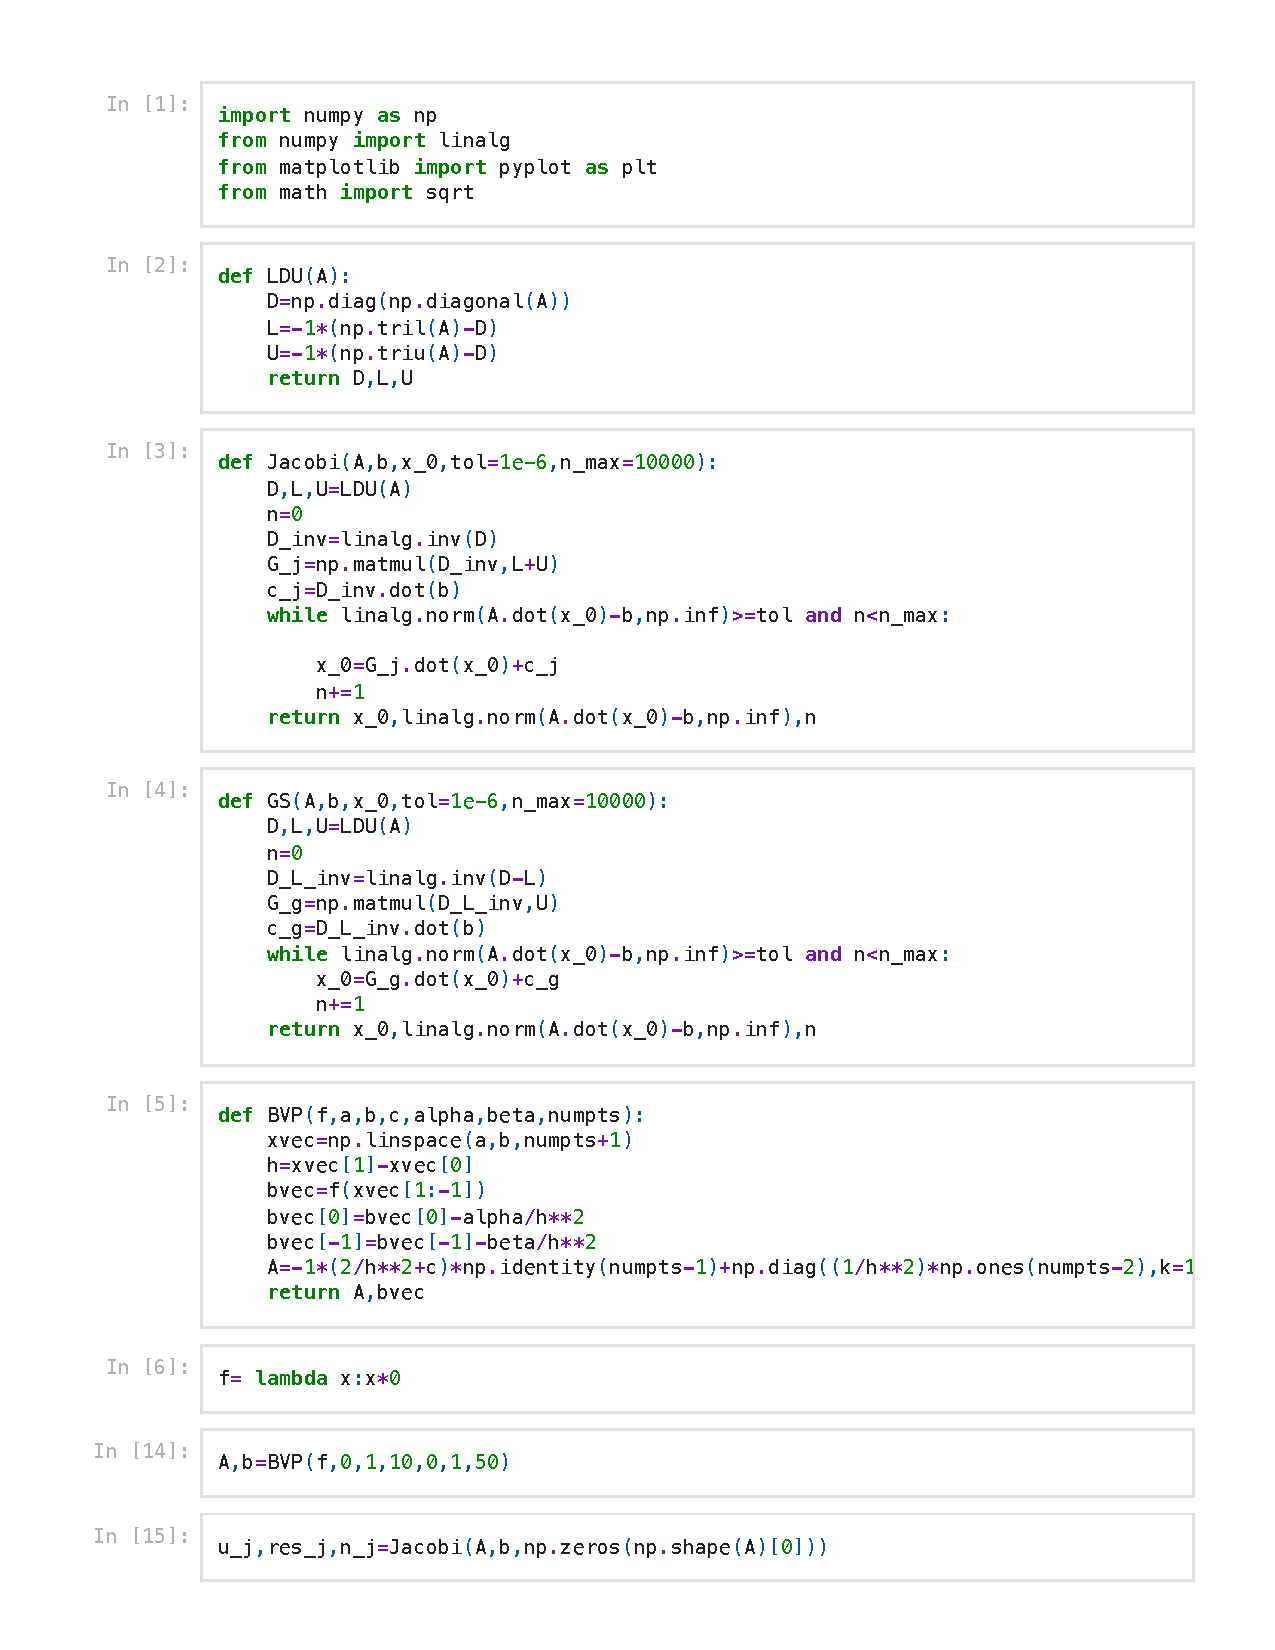
\includepdf[pages=-]{hw_7_151b_2.pdf}
\end{document}